\DocumentMetadata{
    tagging=on,
    tagging-setup={math/setup=mathml-SE},
    pdfstandard=ua-2,
    lang=en-US,
}
\documentclass[11pt,english]{article}



\listfiles
\usepackage{fullpage}
\usepackage[showframe=false,margin=1in]{geometry}
\parindent=0pt

\usepackage{relsize}
\usepackage[T1]{fontenc} % for properly hyphenating words with accented chars
\usepackage{babel}

\usepackage{epsfig}
\usepackage{graphicx}
\usepackage{wrapfig}
\usepackage[belowskip=0pt,aboveskip=0pt,font=small]{caption}
\usepackage{subcaption}
\setlength{\intextsep}{7pt plus 0pt minus 0pt}

\usepackage{amsmath, amsthm, amssymb}
\usepackage{textcomp}
\usepackage{stmaryrd}
\usepackage{upgreek}
\usepackage{bm}
\usepackage{cases}
\usepackage{mathtools}

\usepackage{url}
\usepackage{breakurl}
\usepackage[colorlinks=true]{hyperref}
\usepackage{xspace}
\usepackage{comment}
\usepackage{color}
\usepackage{afterpage}
\usepackage[normalem]{ulem}
\usepackage{enumitem}



\usepackage{../assets/mysymbols}
\usepackage{amsmath,amsfonts}
\usepackage{amsthm,amssymb,amsopn}
\usepackage{bm} % bold symbol
\usepackage{bbm}

\newcommand{\vct}[1]{\boldsymbol{#1}} % vector
\newcommand{\mat}[1]{\boldsymbol{#1}} % matrix

\newcommand{\field}[1]{\mathbb{#1}}
\newcommand{\R}{\field{R}} % real domain
\newcommand{\C}{\field{C}} % complex domain
\newcommand{\F}{\field{F}} % functional domain
\newcommand{\T}{^{\textrm T}} % transpose
\newcommand{\TN}{^{-\textrm T}} % transpose
\newcommand{\Lagr}{\mathcal{L}}


\newcommand{\cst}[1]{\mathsf{#1}}

\newcommand{\inner}[2]{#1\cdot #2}
\newcommand{\twonorm}[1]{\|#1\|_2^2}
\newcommand{\Map}[1]{\mathcal{#1}}

\newcommand{\ProbOpr}[1]{\mathbb{#1}}
\newcommand\independent{\protect\mathpalette{\protect\independenT}{\perp}}
\def\independenT#1#2{\mathrel{\rlap{$#1#2$}\mkern2mu{#1#2}}}
\newcommand{\cind}[3]{{#1} \independent{#2}\,|\,#3}
\newcommand{\cndexp}[2]{\ProbOpr{E}\,[ #1\,|\,#2\,]}



\newtheorem{thm}{Theorem}

\newcommand{\eat}[1]{}

\newcommand{\hide}[1]{}

\newcommand{\diff}{\mathop{}\!\mathrm{d}}
\newcommand{\Vop}{\textrm{T}}
\newcommand{\norminf}[1]{\norm{#1}_\infty}

\newcommand{\vecy}{\ensuremath{\mathbf{y}}\xspace}
\newcommand{\vecx}{\ensuremath{\mathbf{x}}\xspace}
\renewcommand{\argmax}{\operatornamewithlimits{argmax}}
\newcommand{\startsym}{\mbox{\scriptsize \texttt{<s>}}\xspace}
\newcommand{\stopsym}{\mbox{\scriptsize \texttt{</s>}}\xspace}
\newcommand{\best}{\ensuremath{\mathit{best}}\xspace}
\newcommand{\bestuptoi}{\ensuremath{\texttt{best}_{\leq i}}\xspace}
\newcommand{\bestuptot}{\ensuremath{\texttt{best}_{\leq t}}\xspace}
\newcommand{\completed}{\ensuremath{\texttt{comp}}\xspace}
\newcommand{\toptop}{\operatornamewithlimits{\mathbf{top}}}
\newcommand{\tuple}[1]{\ensuremath{\langle {#1} \rangle}}
\newcommand{\xuptot}{\ensuremath{\mathit{x}_{\leq t}}\xspace}


\renewcommand{\hide}[1]{}

\begin{document}
\title{CS 4644/7643: Deep Learning\\
Fall 2026 \\
Problem Set 4}

\author{Instructor: Danfei Xu \\
TAs: Rohan Bansal, Uzu (Chris) Lee, Alfred Cueva  \\
Kun-Lin Hsieh, Chuye Zhang, Liqian Ma, Robert Azarcon  \\
Dhruv Ahuja, Xinchen Yin \\
Discussions: \url{https://piazza.com/class/ms43b2tjxa63lq\#}}
\date{Due: November 16, 2026, 11:59pm}
\maketitle

\paragraph*{Instructions}
\begin{enumerate}
\item We will be using Gradescope to collect your assignments.  Please read the following instructions for submitting to Gradescope carefully!
    \begin{itemize}
        \item
               For the \textbf{HW4 Theory} component on Gradescope, upload one single PDF containing the answers to all the theory questions. \textbf{However, the solution to each problem/subproblem must be on a separate page. When submitting to Gradescope, please make sure to mark the page(s) corresponding to each problem/sub-problem.} Questions with misassigned pages will be penalized by up to 1 point.
          \item
               For the \textbf{HW4 Code} on Gradescope, please use the \texttt{collect\_submission.py} script provided and upload \textbf{hw4\_code\_submission.zip}
          \item
               For the \textbf{HW4 Notebook} component on Gradescope, please use the \texttt{collect\_submission.py} script provided and upload the resulting \textbf{hw4\_notebook\_submission.pdf} on Gradescope.
          \item
               Note: This is a large class and Gradescope's assignment segmentation features are essential.
               Failure to follow these instructions may result in parts of your assignment being penalized.
               We will not entertain regrading requests for failure to follow instructions.
        
    \end{itemize}

    \item
    \LaTeX'd  solutions are strongly encouraged,
    but scanned handwritten copies are acceptable.
    Hard copies are \textbf{not} accepted.

    \item We generally encourage you to collaborate with other students.
    
    You may talk to a friend,
    discuss the questions and potential directions for solving them. However, you need to write
    your own solutions and code separately, and \emph{not} as a group activity.
    Please list the students you collaborated with. \\ \\

\end{enumerate}



\section{Collaborators [0.5 points]}
Please list your collaborators and assign this list to the corresponding section of the outline on Gradescope. If you don't have any collaborators, please write 'None' and assign it to the corresponding section of the Gradescope submission regardless. Not assigning this question on Gradescope or leaving it blank will be marked as zero.

\newpage
\section{Variational Auto-Encoders}

\begin{figure}[h]
  \centering
  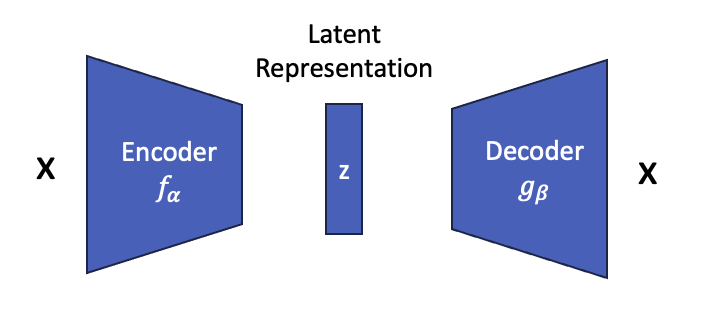
\includegraphics[width=0.5\textwidth, alt={Standard auto-encoder that takes an input x, encodes it into a latent representation z, and then decodes back into the original x.}]{assets/auto-encoder.png}
  \caption{Standard auto-encoder that takes an input $x$, encodes it into a latent representation $z$, and then decodes back into the original $x$. }
  \label{fig:your_label}
\end{figure}

Variational Auto-Encoders (VAE) are latent variable models that can generate samples from a target distribution. Unlike standard autoencoders, VAEs learn a structured latent space that we can reliably sample from to generate new data. This problem walks you through deriving the ELBO training objective for VAEs.

\begin{enumerate}
    \item \textbf{Understanding the ELBO [3 points + 1 point required for 7643/extra-credit for 4644]}
    
    Given a dataset $X$, we want to model the underlying distribution $p(x)$. A latent variable model assumes each observation $x$ is generated from a lower-dimensional latent code $z$: first sample $z \sim p(z)$, then generate $x \sim p_\theta(x|z)$. Here $p(z)$ is a fixed prior (typically $\mathcal{N}(0, I)$) and $p_\theta(x|z)$ is a learned conditional distribution parameterized by $\theta$. 
    For our training objective, we wish to maximize the marginal log-likelihood:
    \[
    \log p_\theta(x) = \log \int p_\theta(x, z)\,dz = \log \int p_\theta(x|z)p(z)\,dz.
    \]
    \noindent However, computing this integral is intractable for deep latent variable models: there is no closed-form solution, and numerical integration over high-dimensional latent spaces is prohibitively expensive. To handle this intractability, we introduce an approximate posterior distribution $q_\phi(z|x)$ that we can tractably compute and sample from.
    \begin{enumerate}
      \item \textit{Deriving the ELBO.} [2 pts]
      
      Derive a tractable lower bound on the log-likelihood by introducing the approximate posterior $q_\phi(z|x)$. Show that:
        \[
            \mathcal{L}(\theta, \phi; x) := \mathbb{E}_{z \sim q_\phi(z|x)}\left[\log \frac{p_\theta(x, z)}{q_\phi(z|x)}\right] \leq \log p_\theta(x)
        \]
        This quantity $\mathcal{L}(\theta, \phi; x)$ is called the Evidence Lower Bound (ELBO). Any mathematically correct derivation is acceptable: Jensen's inequality, KL-divergence properties, etc.
    
    
        Some helpful identities:
        \[
        \log p_\theta(x) = \int q_\phi(z|x) \log p_\theta(x) dz = \mathbb{E}_{z \sim q_\phi(z|x)}[\log p_\theta(x)]
        \qquad
        \frac{q_\phi(z|x)}{q_\phi(z|x)} = 1
        \]
        
      \item \textit{Decomposing the objective.} [1 pt]

        Using the identity
        \[
        \log p_\theta(x) = \mathcal{L}(\theta,\phi;x) 
            + D_{KL}(q_\phi(z|x) \,\Vert\, p_\theta(z|x)),
        \]
        explain why maximizing $\mathcal{L}(\theta,\phi;x)$ with respect to $\phi$
        is equivalent to minimizing $D_{KL}(q_\phi(z|x)\,\Vert\, p_\theta(z|x))$.
        Why can't we minimize this KL directly instead of maximizing the ELBO?
        
      \item \textit{Understanding the ELBO terms.} [1 pt] \textbf{(Required for 7643; Extra Credit for 4644)}

        From part (a), the ELBO can be rewritten as:
        \[
        \mathcal{L}(\theta, \phi; x) 
            = \underbrace{\mathbb{E}_{z \sim q_\phi(z|x)}[\log p_\theta(x|z)]}_{\text{reconstruction term}}
            - \underbrace{D_{KL}(q_\phi(z|x) \,\Vert\, p(z))}_{\text{regularization term}}
        \]
        Suppose we train a VAE but remove the KL term entirely, optimizing only
        $\mathbb{E}_{z \sim q_\phi(z|x)}[\log p_\theta(x|z)]$. What is one degenerate distribution $q_\phi(z|x)$ could collapse to? Why would this break generation at test time, even if reconstruction loss is low?

    \end{enumerate}

    \item \textbf{Reparameterization Trick [1 point]}
    
    To train the VAE using gradient descent, we need to compute gradients of the ELBO with respect to both $\theta$ and $\phi$:
    \[
    \mathcal{L}(\theta, \phi; x) = \mathbb{E}_{z \sim q_\phi(z|x)}[\log p_\theta(x|z)] - D_{KL}(q_\phi(z|x) \,\Vert\, p(z))
    \]
    
    \begin{enumerate}
        \item \textit{The reparameterization trick.} [1 pt]
        
        For $q_\phi(z|x) = \mathcal{N}(\mu_\phi(x), \sigma_\phi^2(x)I)$, instead of sampling $z \sim q_\phi(z|x)$ directly, we:
        \begin{enumerate}
            \item Sample $\epsilon \sim \mathcal{N}(0, I)$
            \item Compute $z = \mu_\phi(x) + \sigma_\phi(x) \odot \epsilon$
        \end{enumerate}
        
        This gives us:
        \[
        \mathbb{E}_{z \sim q_\phi(z|x)}[\log p_\theta(x|z)] = \mathbb{E}_{\epsilon \sim \mathcal{N}(0,I)}[\log p_\theta(x|\mu_\phi(x) + \sigma_\phi(x) \odot \epsilon)]
        \]
        
        Explain why this solves the gradient problem. Why can we now move $\nabla_\phi$ inside the expectation?
        
    \end{enumerate}

\end{enumerate}


\newpage
\section{Diffusion Models}

\begin{enumerate}
\item
    Before starting section, we highly recommend reading the \href{https://arxiv.org/abs/2006.11239}{DDPM} paper to familiarize yourself with the notation and equations.
    
    Denoising Diffusion Probabilistic Models (DDPMs) learn to reverse a gradual noising process. The forward process transforms data $x_0 \sim q(x_0)$ into noise through $T$ steps, defined as a Markov chain:
    \[
    q(x_{1:T} | x_0) = \prod_{t=1}^T q(x_t | x_{t-1})
    \]
    where each transition adds Gaussian noise:
    \[
    q(x_t | x_{t-1}) = \mathcal{N}(x_t; \sqrt{\alpha_t} x_{t-1}, \beta_t I).
    \]
    
    The goal is to learn a \textbf{reverse process} $p_\theta$ that inverts this noising:
    \[
    p_\theta(x_{0:T}) = p(x_T) \prod_{t=1}^T p_\theta(x_{t-1} | x_t)
    \]
    where $p(x_T) = \mathcal{N}(x_T; 0, I)$ and we model each reverse step as:
    \[
    p_\theta(x_{t-1} | x_t) = \mathcal{N}(x_{t-1}; \mu_\theta(x_t, t), \Sigma_\theta(x_t, t)).
    \]
    Starting from noise $x_T \sim \mathcal{N}(0, I)$ and iteratively sampling from $p_\theta(x_{t-1} | x_t)$, we can generate new data samples.
    
    The framework makes some key assumptions:
    \begin{enumerate}
        \item \textbf{Markov property}: $q(x_t | x_{t-1}, \ldots, x_0) = q(x_t | x_{t-1})$ --- each step depends only on the previous timestep.
        \item \textbf{Gaussian transitions with fixed schedule}: $\{\beta_t\}_{t=1}^T$ is predetermined with $0 < \beta_1 < \beta_2 < \cdots < \beta_T < 1$.
        \item \textbf{Small noise per step}: When $\beta_t$ is sufficiently small, the reverse process posterior $q(x_{t-1} | x_t)$ is approximately Gaussian \href{https://arxiv.org/abs/1503.03585}{(Sohl-Dickstein et al., 2015)}. This is why DDPMs model the reverse process $p_\theta(x_{t-1} | x_t)$ as a Gaussian.
    \end{enumerate}

\item \textbf{Forward diffusion [3 points]}
    Define the noise schedule $\{\beta_t\}_{t=1}^T$ with $\alpha_t=1-\beta_t$ and $\bar\alpha_t=\prod_{s=1}^t \alpha_s$. The forward process is
    \[
    q(x_t\mid x_{t-1})=\mathcal N(\sqrt{\alpha_t}\,x_{t-1},\,\beta_t I).
    \]
    Equation 4 in the DDPM paper gives a closed form expression for the forward process at an arbitrary timestep $t$:
    \[
    q(x_t\mid x_0)=\mathcal N\!\Big(\sqrt{\bar\alpha_t}\,x_0,\ (1-\bar\alpha_t)I\Big).
    \]
    \begin{enumerate}
        
        \item \textit{Closed form of $q(x_t|x_0)$} [2 pt]
        
        Prove the expression above for $q(x_t|x_0)$ is true for all $t\geq 1$ by induction on $t$. 
        
        \textbf{Helpful identities:}
        \begin{itemize}
            \item \textit{Reparametrization trick}: A random variable $X \sim \mathcal{N}(\mu, \sigma^2 I)$ can be written as $X = \mu + \sigma \epsilon$ where $\epsilon \sim \mathcal{N}(0, I)$.
            \item \textit{Sum of independent Gaussians}: If $X \sim \mathcal{N}(0, I)$ and $Y \sim \mathcal{N}(0, I)$ are independent, then $aX + bY \sim \mathcal{N}(0, (a^2 + b^2)I)$, or equivalently $aX + bY = \sqrt{a^2 + b^2}\,\epsilon$ where $\epsilon \sim \mathcal{N}(0, I)$.
        \end{itemize}
        
        \item \textit{Noise distribution $q(x_T|x_0)$} [1 pt]
        
        In diffusion models, we choose $\{\beta_t\}$ such that $\bar\alpha_T \approx 0$. What is $q(x_T|x_0)$ when $\bar\alpha_T = 0$? Why is this useful for generation?
    \end{enumerate}


\item \textbf{Reverse Process [2 points + 1 point required for 7643/extra-credit for 4644]}    
    \begin{enumerate}
    
        \item \textit{KL divergence between Gaussians} [1 pt]
        
        Recall that the PDF of a univariate Gaussian $\mathcal{N}(\mu, \sigma^2)$ is:
        \[p(x) = \frac{1}{\sqrt{2\pi\sigma^2}} \exp\left(-\frac{(x - \mu)^2}{2\sigma^2}\right)\]
        
        and the KL divergence between two distributions $p$ and $q$ is:
        \[D_{KL}(p \| q) = \mathbb{E}_{x \sim p}\left[\log \frac{p(x)}{q(x)}\right]\]
        
        Show that when $p = \mathcal{N}(\mu_1, \sigma^2)$ and $q = \mathcal{N}(\mu_2, \sigma^2)$ share the same variance:
        \[D_{KL}(\mathcal{N}(\mu_1, \sigma^2) \| \mathcal{N}(\mu_2, \sigma^2)) = \frac{1}{2\sigma^2}(\mu_1 - \mu_2)^2\]

    
        \item \textit{Connecting to DDPM} [1 pt]
        
        Using the result from part (a), explain in 1-2 sentences why $L_{t-1} = D_{KL}(q(x_{t-1}|x_t,x_0) \| p_\theta(x_{t-1}|x_t))$ simplifies to:
        \[L_{t-1} = \mathbb{E}_q\left[\frac{1}{2\sigma_t^2}\|\tilde\mu_t(x_t,x_0) - \mu_\theta(x_t,t)\|^2\right] + C\]
        What key assumption on $p_\theta$ makes part (a) applicable?


        \item \textit{Forward process posterior} 
        [1 point] \textbf{(Required for 7643; Extra Credit for 4644)}: 

        In Appendix A, the authors rewrite the $q(x_{t-1}|x_t)$ terms as $q(x_{t-1}|x_t,x_0)$. Why can't we compute $q(x_{t-1}|x_t)$? Why is $q(x_{t-1}|x_t,x_0)$ a valid substitution?
    \end{enumerate}

\end{enumerate}

\newpage
\section{Paper Review [2 Points]}
For this homework, you'll be writing a paper review for \textbf{Denoising Diffusion Probabilistic Models}.  We recommend reading this paper before you start the theory and coding sections on diffusion models. 

The paper introduces a method for high quality image generation inspired by non-equilibrium thermodynamics. Diffusion models operate through a forward noising process and a reverse denoising process.  These state of the art generative models are useful in many domains including image generation and robotics. The paper can be viewed \href{https://arxiv.org/abs/2006.11239}{here}.

\vspace{2mm}
The review will be graded using the following evaluation rubric:
\begin{enumerate}
\item
\textbf{[1 point]}
Briefly summarize the key contributions, strengths and weaknesses of this paper.

\item
\textbf{[1 point]}
What is your personal takeaway from this paper? 

\end{enumerate}

Guidelines: Please restrict your reviews to at least one paragraph per question, but no more than 350 words (total length for answers to both of the above questions). Please write separate answers for each question to assist in Gradescope grading.

\end{document}